\chapter{Manual de utilización}
\label{Anexo:manualuso}

Como se ha explicado, existen dos formas de ejecutar la aplicación. 

La primera, un script el cual contiene un comando de ayuda(en el caso de ejecutar sin parámetros) que muestra una lista de los argumentos disponibles para lanzar el programa. Es importante recalcar que, pese a que el script es automático, algunas de las tareas como el envío de e-mails, requieren del usuario para rellenar los campos de texto en el momento de la ejecución.

En el caso del \textit{main} con interacción por parte del usuario el funcionamiento es el siguiente:

El sistema pide al usuario elegir entre las 3 opciones iniciales.
\begin{enumerate}
	\item {Envío y recibo de e-mails anónimos(sección de \textit{mailing}).}
	
	\item {Automatización de log-in, registro y diversas tareas(sección de \textit{accounts})}.
	
	\item {Visualización de la base de datos de accounts en un servicio oculto con \textbf{Tor}}.
\end{enumerate}


\begin{figure}[h]
	\centerline{
		\mbox{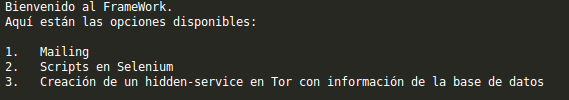
\includegraphics[width=5.00in]{images/menu_ini.png}}
	}
	\caption{Menú principal de la herramienta (modo interfaz)}
	\label{fig:inicial}
\end{figure}

En el caso de elegir la primera opción, se permite elegir entre el \textbf{remailer}, la \textbf{bandeja de entrada temporal} o el \textbf{mailer} con posibilidad de ofuscar la estilometría.


\begin{figure}[h]
	\centerline{
		\mbox{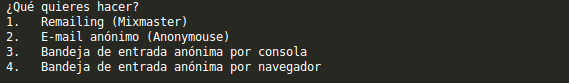
\includegraphics[width=5.00in]{images/mailing.png}}
	}
	\caption{Menú de la sección de \textit{mailing} de la herramienta (modo interfaz)}
	\label{fig:mailing}
\end{figure}

En el caso de elegir la segunda opción, se dará a elegir al usuario en cuál de los servicios disponibles (periódico online, redes sociales, foro de discusión\dots) desea realizar una tarea. Dichas tareas son \textbf{registro automático, inicio de sesión automático, o realización de tarea sencilla(dependiendo de la página)}.

\begin{figure}[h]
	\centerline{
		\mbox{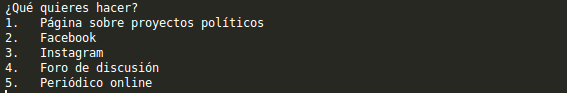
\includegraphics[width=5.00in]{images/accounts.png}}
	}
	\caption{Menú de la sección de \textit{accounts} de la herramienta (modo interfaz)}
	\label{fig:accounts}
\end{figure}

\begin{figure}[h]
	\centerline{
		\mbox{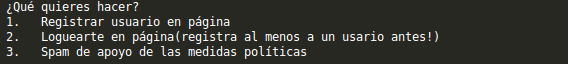
\includegraphics[width=5.00in]{images/medidas_politicas.png}}
	}
	\caption{Opciones disponibles en una página web en la sección de \textit{accounts}}
	\label{fig:medidas}
\end{figure}

\begin{figure}[h]
	\centerline{
		\mbox{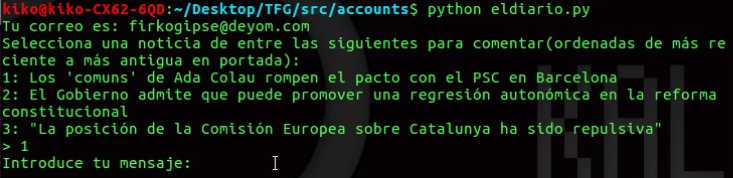
\includegraphics[width=5.00in]{images/eldiario.png}}
	}
	\caption{Ejemplo de acción automática, en este caso, en un periódico de opinión (usando Tor como \textit{WebDriver})}
	\label{fig:eldiario}
\end{figure}


Por último, la tercera opción muestra una dirección .onion donde estará disponible la base de datos hasta el momento en el que la instancia del programa se cierre.

\newpage \thispagestyle{empty} % Página vacía 